\todo{predelat na spravny format pdf}
\todo{zeptat se na odkazy u obrazku a odkazy u FANN a URHO3D}
\todo{vytvorit apendix}
\todo{ma byt intorduction chapter s cislem?}

\chapter{Introduction}
Magic has always been a popular part of computer games. In many games, magic has its own lore and laws that make it systematical. Great examples of the complexity of magical spell systems include the games \emph{Magicka} and \emph{Magicka 2}, where the player casts spells by combining eight elements (as seen on \cref{fig:magicka}): For example, using only earth element results in a rock thrown at the enemy, but adding fire will create a classic fireball.

\begin{figure}
  \centering
  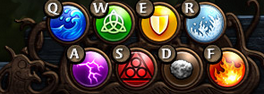
\includegraphics[width=0.5\textwidth]{ext/magicka.png}
  \caption{\emph{Magicka} spell interface}
  \label{fig:magicka}
\end{figure}

In books and movies, wizards can be seen performing complicated hand gestures or drawing complex shapes in order to cast spells. In games, on the other hand, casting magic is usually extremely easy, since players may often just push a few buttons to cast even the strongest spells. This spoils the feeling of magic as something extraordinary and secret, requiring years of study. Complicated magic systems allow the game developers to engage players in a different game experience, requiring focus, some amount of creative thinking, and possibly cooperation with other players.

In this thesis, we focus on the constructive kind of spell casting: While the majority of games simply binds spells to buttons, there are several that use some kind of different system. One class of such systems uses pattern recognition algorithms to translate the player's image-like (or, say, rune-like) input to a spell definition. However, as shown in the next section, these systems usually recognize only simple gestures or patterns, which is partly caused by the difficulties in implementing such a system\footnote{In this thesis we ignore other difficulties, which mainly include various marketing and accessibility issues.}. The goal of this thesis is to create a comprehensive pattern recognition system that can be easily plugged into games to allow simple and robust recognition of player-drawn shapes and their translation to an arbitrary spell system.

\section{Pattern recognition in current games}

Symbols and gestures are usually an integral part of the magic and there were many attempts to bring them into video game environment. \citet{gameMagic} provides a classification of existing gestural systems into three categories (which sometimes overlap and combination of these approaches is used):

\begin{description}
\item[Alternative controllers]
One such category are systems that utilize alternative controllers to mouse and keyboard, such as Wiimote Kinect. A recent game from this category is \emph{Fable: The Journey}, where the player casts spells by moving his hands: For example, push spell is cast by pushing into the air. Patterns made by the player are recognized using Kinect technology. While moves are simple in nature, such as waving sideways or back and forth, both hands at the same time can be used, which results in quite complex gestures.

\item[Restricted drawing forms]
Another technique used in several games is to let player draw into a predefined grid, or through predefined points. Both \emph{Castlevania: Dawn of Sorrow} and \emph{Deep Labyrinth} take advantage of an Nintendo DS drawing interface that allows players to draw magic signs. 
In \emph{Castlevania}, players draw signs by connecting glowing points in a circle in out-of-combat situations, as seen in \cref{fig:castlevania}. \emph{Deep Labyrinth} introduces special casting interface that consists of $3\times 3$-grid, where the player connects dots.

The restriction to pre-existing following grid takes away a part of the creative freedom, but makes recognition algorithms much easier to implement and run: For example, only tracing the order of the connected points in \emph{Deep Labyrinth} is sufficient to recognize the spell.

\begin{figure}
\centering
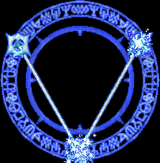
\includegraphics[width=.3\linewidth]{ext/castlevania.png}
\quad
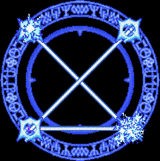
\includegraphics[width=.3\linewidth]{ext/castlevania2.png}
\caption{\emph{Castlevania: Dawn of Sorrow} spell interface \XX{(image taken from ?)}}
\label{fig:castlevania} %label se vaze na caption a musi bejt az po nem
\end{figure}

\item[Free-hand drawing]
One of the first games to integrate some form of pattern recognition of drawn shapes is \emph{Black \& White}. Using a mouse, players are able to cast miracles by drawing a specific pattern on the ground, as in \cref{fig:blackwhite}. The player can draw anything anywhere on the ground, and its up to the game logic to recognize if the result matches some of the miracle patterns. Alternatively, the player can still cast miracle by clicking on a button --- presumably because a lot of players had trouble drawing the miracles.

A similar approach to recognition of player-drawn spells is used in \emph{Arx Fatalis}. Players are drawing symbols into the air with a mouse, and a sequence of the drawn symbols represents some spell. While casting, game encodes the mouse moves into characters that represent the 8 directions. After player finishes the spell, a Levenshtein distance is calculated from each predefined spell sequence to the player's created sequence and the candidate with the lowest Levenshtein cost is returned as a matching spell.

\begin{figure}
\centering
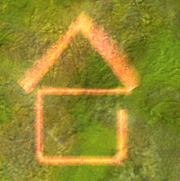
\includegraphics[width=.3\linewidth]{ext/gestureteleport.png}
\quad
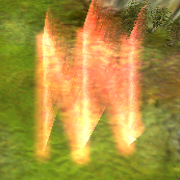
\includegraphics[width=.3\linewidth]{ext/gesturefireball.png}
\caption{\emph{Black \& White} teleport and fireball gestures}
\label{fig:blackwhite}
\end{figure}

\end{description}

\section{Goals}

The result of the thesis allows the players to draw complex spells, preferably more complex than in \emph{Black\&White} or \emph{Arx Fatalis}. For that purpose, we create an algorithm that recognizes a set of basic symbols which can be arbitrarily combined to form new, very complex symbols.

Possibilities of such combinations include composition (symbol is made from other smaller symbols) and embedding (a symbol is put inside another symbol, or into a somehow important position relative to other symbol, e.g. on the top of a triangle). Several examples of symbols and their combinations is shown in \cref{fig:examples}.

\begin{figure}[p]
\centering
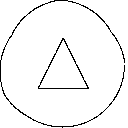
\includegraphics[width=.3\linewidth]{ext/images/embedd.png}
\quad
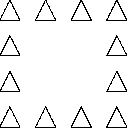
\includegraphics[width=.3\linewidth]{ext/images/comp.png}
\quad
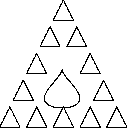
\includegraphics[width=.3\linewidth]{ext/images/comp_and_embed.png}

\vspace{1cm}

\centering
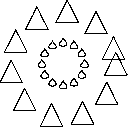
\includegraphics[width=.3\linewidth]{ext/images/comp_in_comp.png}
\quad
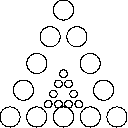
\includegraphics[width=.3\linewidth]{ext/images/comp_in_comp2.png}
\quad
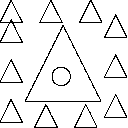
\includegraphics[width=.3\linewidth]{ext/images/triple.png}
\caption{In the figure, embedded positions are always in the middle of the shape. From left to right: circle with embedded triangle; square composed of triangle; triangle composed of triangle, with water drop embedded; circle composed of triangles, with embedded circle composed of water drop; triangle composed of circle, with embedded triangle composed of circle; square composed of triangle, with embedded triangle, with embedded circle in the triangle}
\label{fig:examples}
\end{figure}


We refrain from using any aiding structures (as e.g. in \emph{Castlevania}) to retain generality of the system.

For the purpose of evaluation the work, we specify the following requirements on the resulting recognition system:
\begin{description}

\item [Durability against shape deformations]
Since we want to recognize hand-drawn shapes, our system has to be prepared for human-like imprecise drawing, especially when drawing with a mouse. However, drawing an exact line between a shape that should still be recognized and a shape that should be rejected is difficult and possibly subjective; we therefore only evaluate the performance on deformed shapes.

\item [Extensibility]
We would like to offer an easy-to-use library that can be utilitized in other projects. For this purpose, we need to let the users define their own shapes that should be recognized. The library should provide interfaces for both preparing custom shapes and using them in the pattern recognition.

\item [Performance]
Our system should be applicable in demanding video games environment, prepared for the possibility of many players drawing their spells at once. To achieve this, we require fast recognition technique preferably usable in a parallel environment.

\item [Recognition of embedded shapes]
To allow players cast complex spells, we need to give them an ability to somehow encode multiple symbols in one spell. One possible way to do it are shape embeddings. Each defined shape can contain several areas, where other shapes might occur. These areas are then processed in our recognition system and classified.

\item [Recognition of shape conglomerations]
For the purpose of this work, we consider shape conglomeration a group of shapes from the same shape class e.g. circle, arranged such that the whole conglomeration forms another shape. We can also look at it as taking the curves of the shape, sampling them uniformly, and then replacing all the samples with the pattern shape.
\end{description}

\subsection{Approach}
The thesis is divided into several steps: First chapter reviews the approaches and algorithms commonly used to solve the pattern recognition problem. We have closely examined three algorithms, namely the \emph{Normalized cross-correlation},\emph{Shape matching and object recognition using shape contexts} and \emph{Matching of Shapes Using Dynamic Programming}. In the same chapter, we describe \emph{Artificial neural networks} and place them in the context of pattern recognition. In \cref{ch:impl}, we describe the implementation of the resulting neural-network-based recognition algorithm. The implementation is accompanied by a simple game prototype that is used to demonstrate the properties of the recognition system. Finally, we perform benchmarking of the performance of our algorithm, with respect to recognition success rate and speed.

In the appendix, we describe the interface of our algorithm and provide a guide for using it in another project. A simple explanation of demonstrational game usage is also included.
